We describe the process of removing NaNs, removing cross-correlated features, special treatment of categorical variables and standardization of data.

\subsection{Dealing with NaNs}
As decribed in the CERN document~\cite{cern-doc}, some features may have \emph{missing data} in the form of the value -999.0, which is not valid for any feature.
The approach we test here for dealing with such data is, for each observation in which at least one feature has an invalid value, to remove the whole observation from the dataset.
Applying the process to the training dataset yields a drop in the number of samples of 72\%, i.e. from a total observation count of $2.5 \times 10^5$ to $6.8 \times 10^4$ observations, suggesting that this method is perhaps too consevative.
Surprisingly, not removing the invalid observations yields slightly better solutions in the classification process.
This suggests that it might be worth it to investigate more sophisticated methods of dealing with NaNs, such as assigning missing values to their nearest neighbours.

\subsection{Cross-correlated features}
Some features present a high degree of cross-correlation.
Not only is it more convenient to remove them from a computational point of view, but it can also be better for the numerical stability of some ML algorithms.  \\
%\begin{figure}
%\centering
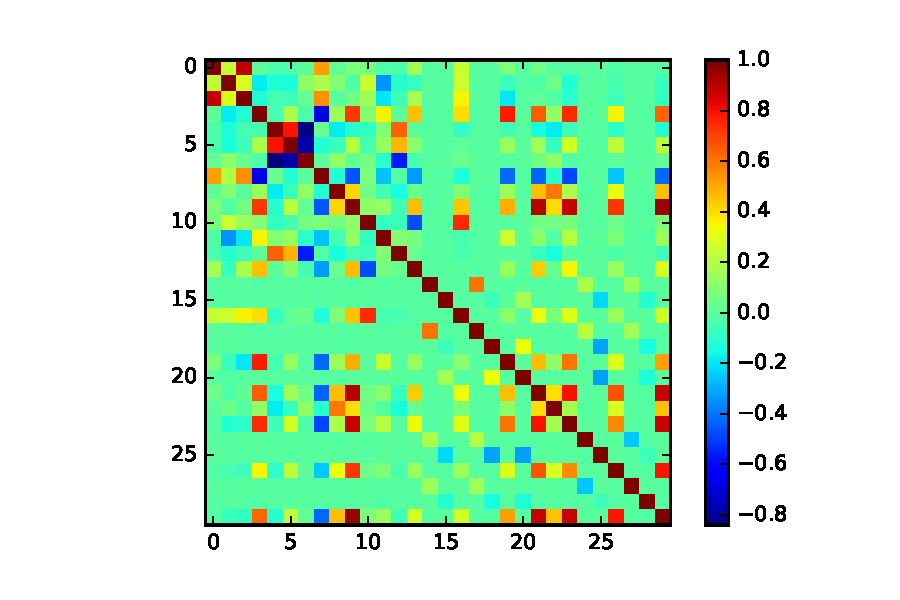
\includegraphics[width=0.8\columnwidth]{corr-coef-matrix.pdf}
\captionof{figure}{Matrix of correlation coefficients. \label{fig-corr}}
%\end{figure}
We analyzed the correlation coefficient matrix in Figure~\ref{fig-corr} and decided to remove feature number 9 (i.e. \texttt{DER\_sum\_pt}) because it is a derived feature with a high correlation ($> 0.95$) to the primary feature number 29 (i.e. \texttt{PRI\_jet\_all\_pt}).

\subsection{Categorical variables}
Analysis of the CERN document~\cite{cern-doc} reveals that one feature, namely \texttt{PRI\_jet\_num}, only takes integer values $0,1,2,3$.
As these represent actual quantities, it is arguable whether this should be treated as a categorical variable or not.
However, since some of the derived features appear to have different formulas according to the value of \texttt{PRI\_jet\_num} we argue that this should be treated as a categorical variable.
As such, we define as customary a set of dummy variables, each one associated to the possible levels of \texttt{PRI\_jet\_num}, that take the value 1 for the observations where \texttt{PRI\_jet\_num} is equal to that level, and 0 otherwise.

\subsection{Standardization of data}
The values taken by different features can vary wildly and take quite large values which can cause overflow problems, thus a normalization procedure is necessary.
We opt for a normalization based on computing the eigendecomposition of the covariance matris of the centered data matrix $X - \bar{X}$:
\begin{equation}
\text{compute } \Lambda, U \text{ such that: } (X - \bar{X}) = U\Lambda U^T.
\end{equation}
This transformation yields the whitened data $X_w$:
\begin{equation}
X_w = \Lambda^{-1/2}U^T(X - \bar{X}).
\end{equation}

